\documentclass{article}
\usepackage{tikz}
\usepackage{pgf-umlcd}
\begin{document}
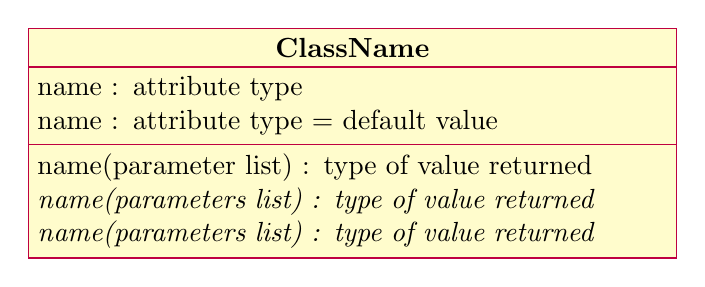
\begin{tikzpicture}
  \begin{class}[text width=8cm]{ClassName}{0,0}
    \attribute{name : attribute type}
    \attribute{name : attribute type = default value}
    
    \operation{name(parameter list) : type of value returned}
    % virtual operations
    \operation[0]{name(parameters list) : type of value returned}
    \operation[0]{name(parameters list) : type of value returned}
  \end{class}
\end{tikzpicture}
\end{document}